\chapter{مقدمه}
به دنبال پیشرفت تکنولوژی در ساخت دوربین‌های عکاسی و ورود دوربین‌های نیمه‌خودکار و خودکار به بازار، تعداد زیادی از کاربران سیستم‌های رایانه‌ای به استفاده از این تکنولوژی در ثبت تصاویر مورد علاقه خود جذب شده‌اند. دقت و کیفیت مطلوب تصویربرداری از یک سو و سهولت استفاده از دوربین‌ از سوی دیگر، باعث شده‌ تعداد تصاویر ثبت شده توسط کاربران به طور روزافزون افزایش یابد؛ به‌طوری‌که امروزه اغلب کاربران، تعداد بی‌شماری از این تصاویر را در گوشی‌های تلفن همراه، تبلت‌ها و رایانه‌های شخصی خود نگه‌داری می‌کنند.
\\
از جمله مشکلاتی که در اثر ایجاد این حجم وسیع از تصاویر بوجود آمده، مشکل مدیریت این تصاویر و یافتن تصاویر خاص بین مجموعه بزرگی از تصاویر موجود، است. از همین‌رو دست‌یابی به سامانه‌ای که بتواند به طور خودکار تمامی این تصاویر را مدیریت نماید، یک نیاز برجسته به شمار می‌رود. ارائه سامانه‌ای که قادر به درک تصاویر و توصیف آن‌ها در قالب جملات زبان طبیعی باشد، بستر مناسبی برای مدیریت تصاویر به طور هوشمند را فراهم می‌نماید.
\\
در این فصل، ابتدا موضوع پژوهش را به طور کامل بیان کرده و اهمیت ارائه راه‌کار مناسبی در این خصوص را ذکر می‌نماییم. سپس نگاهی اجمالی و گذرا بر سیر پژوهش‌های مرتبط با این حوزه انداخته و رویکرد اتخاذ شده برای حل این مساله را بیان می‌کنیم. در انتها خلاصه‌ای از آن‌چه در فصول بعدی این گزارش آمده، مطرح خواهیم نمود.
\section{بیان مساله}

درک تصاویر و توانایی توصیف آن‌ها، کلیدی‌ترین امکان قابل تصور برای سامانه‌های مدیریت هوشمند تصاویر به شمار می‌روند. با وجود سامانه‌ای که بتواند به طور خودکار و هوشمند، شرحی توصیفی متناظر هر تصویر دلخواه ورودی تولید نماید، می‌توان مساله مدیریت تصاویر را به مساله جستجوی میان توصیف تولید شده از تصاویر، کاهش داد. 
\\
سامانه مولد شرح خودکار بر تصاویر، سامانه‌ای است که قادر باشد هر تصویر ورودی، با هر اندازه و از هر منظره و موضوع دلخواه را در قالب جملات زبان طبیعی توصیف نماید. شرح تولید شده برای هر تصویر توسط این سامانه، باید به لحاظ زبانی درست بوده و در معنا، توصیف‌کننده تصویر باشد. این جملات علاوه بر این‌که باید از لحاظ دستور زبان و قواعد نحوی،‌ صحیح باشند، باید به لحاظ معنایی نیز حامل معنای کامل و مرتبط با تصویر ورودی باشند.
\\
برای دست‌یابی به سامانه‌ای که قادر به توصیف تصاویر از موضوعات مختلف باشد، ابتدا باید صحنه به نمایش درآمده در تصویر را به درستی درک کرد. درک صحیح از صحنه، عبارت است از بیان تصویر به نحوی که اطلاعات کلی موجود و هدف اصلی تصویر، واضح و مشخص باشد. علاوه بر این، محتوای تصاویر باید به گونه‌ای بیان گردد که جستجوی تصاویر، بر اساس توصیف تولید شده، به سهولت قابل انجام باشد. 
\\
شکل \ref{fig:smpl} نمونه‌هایی از تصاویر ورودی چنین سامانه‌ای را به همراه خروجی تولید شده توسط آن نمایش می‌دهد. همان‌طور که در این نمونه‌ها مشخص است، تصویر ورودی می‌تواند از هر منظره و موضوع دلخواهی باشد و شرح تولید شده باید شامل جملات صحیح زبانی با معنای متناظر تصویر باشند.
\begin{figure}[h]
	\centering
	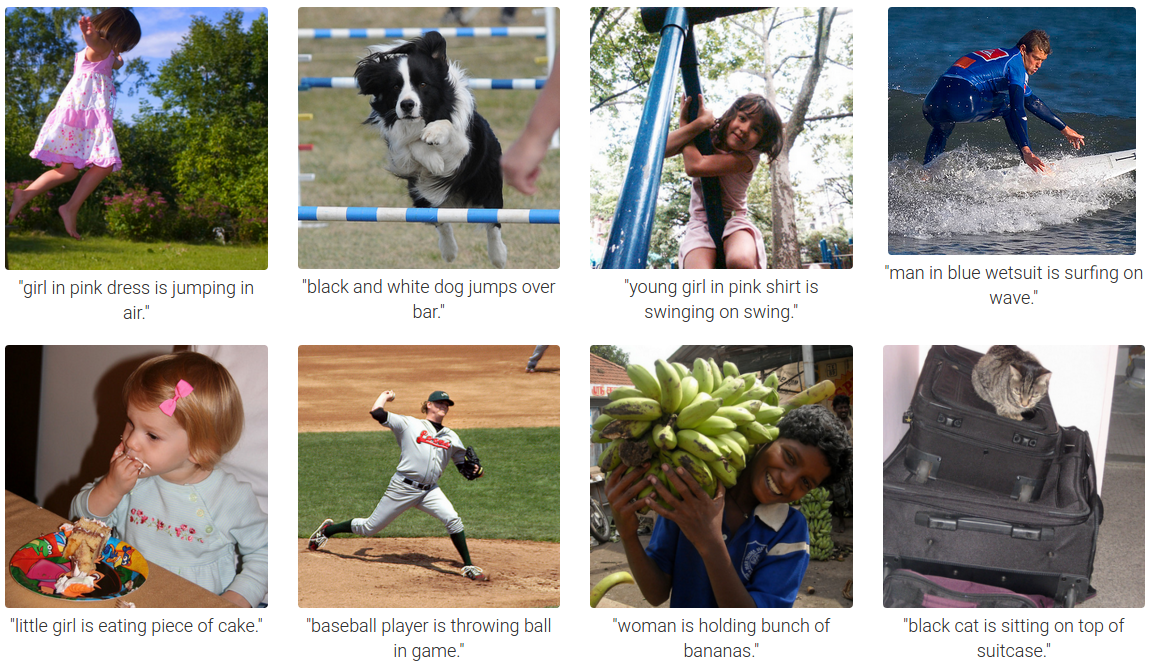
\includegraphics[scale=0.3]{Imgs/CaptionSamples.png}
	\caption{نمونه‌ای از تصاویر ورودی و خروجی‌های مورد انتظار}
	\label{fig:smpl}
\end{figure}

\section{نگاهی بر سیر پژوهش‌های پیشین}

شرح خودکار تصاویر، توجه پژوهش‌گران بسیار زیادی را به خود جلب کرده است و فعالیت‌های متنوع و متعددی در این راستا انجام شده‌اند. نکته قابل تامل در این رابطه، این است که گستره وسیعی از رویکردها و روش‌ها در بین این پژوهش‌ها به چشم می‌خورد. در این بخش از گزارش، نگاهی بر سیر این پژوهش‌ها انداخته و روند پیش‌رفت پژوهش‌ در این حوزه را بیان می‌نماییم.
\\
همان‌طور که بیان شد، ارائه سامانه‌ای که قادر به توصیف تصاویر باشد، نیازمند ارائه روش‌هایی برای حل دو چالش اساسی زیر است.
\begin{enumerate}
	\item چالش درک صحنه 
	(بازنمایی تصاویر با استفاده از بردار ویژگی) \\
	توصیف صحنه باید دقیق باشد؛ به این معنی که اجسام موجود در صحنه باید به طور دقیق از هم تفکیک شده و دسته‌بندی شوند. تصویر توصیف شده باید در قالب مناسبی بازنمایی شود که بتوان به راحتی از آن برای تولید جمله استفاده نمود. استخراج یک یا چند بردار ویژگی مناسب، که اطلاعات مختلف را در خود جای داده‌ باشند، یک بازنمایی مناسب برای تصاویر است.
	\item چالش تولید جمله
	(تبدیل بردار ويژگی به‌دست‌آمده به جملات صحیح زبانی)
	\\
	جملات تولید شده برای شرح تصویر باید به لحاظ دستور زبان، املا و معنا صحیح بوده و با تصویر مرتبط خود سازگار باشند و آن را به درستی و دقت شرح دهند.
\end{enumerate}

در سال‌های قبل از ۲۰۱۴، عموم روش‌های ارائه شده، این دو چالش را به طور مجزا از یک‌دیگر بررسی کرده و ایده یا روش جدیدی برای بهبود یکی از این چالش‌ها ارائه می‌دادند. اما از اواسط سال ۲۰۱۴ به بعد، عموم پژوهش‌گران با اقتباس از روش‌های موجود در حوزه ترجمه ماشینی، با استفاده از یک بستر کاری رمزگذار-رمزگشا\enfootnote{Encoder-Decoder Framework} و با بهره‌گیری از شبکه‌های عصبی کانولوشنی و بازگشتی عمیق، اقدام به ارائه مدل‌های یک‌پارجه برای تولید شرح متناظر تصویر می‌نمایند.
\\
جدول \ref{tbl:smry}، سیر پژوهش‌های مرتبط با حوزه تولید شرح متناظر تصویر را به طور خلاصه نمایش می‌دهد. همان‌طور که در این جدول ملاحظه می‌شود، تا حدود سال ۲۰۰۷ میلادی، پژوهش‌گران در این حوزه، بیشتر روی چالش درک صحنه و استخراج اطلاعات مفید از تصویر تمرکز داشته‌اند. از حدود سال ۲۰۰۷ به بعد، به مرور و با پیشرفت مدل‌های استخراج ویژگی و اطلاعات از تصویر، بخش قابل توجهی از پژوهش‌ها به سمت کار بر روی تولید جملات گرایش پیدا کردند. در سال ۲۰۱۱ با رفع محدودیت یادگیری شبکه‌های عصبی بازگشتی (که در فصل بعد به طور تفصیلی به آن خواهیم پرداخت)، استفاده از روش‌های دیگر برای تولید جمله به کلی کنار گذاشته شد. از حدود سال ۲۰۱۴ میلادی، شبکه‌های عصبی کانولوشنی نیز جایگزین مدل‌های گرافی احتمالی در بخش درک صحنه شدند. از آن پس، عموم پژوهش‌های انجام‌ شده، در بستر کاری رمزگذار-رمزگشا و با استفاده از ترکیب شبکه‌های عصبی کانولوشنی و بازگشتی، اقدام به ارائه مدل‌ها و معماری‌های جدید برای تولید خودکار شرح متناظر تصویر می‌نمایند.

\begin{table}[h]
	\centering
	\caption{خلاصه‌‌ای از سیر پژوهش‌های پیشین در حوزه تولید شرح متناظر تصاویر}
	\label{tbl:smry}
	\begin{tabular}{|c|c|c|}
		\hline
		روش کلی پژوهش در درک صحنه& روش کلی پژوهش در تولید جمله &‌ بازه زمانی
		\\
		\hline
		دسته‌بندی تصاویر & تولید زبان طبیعی & قبل از سال ۲۰۰۰
		\\
		مدل‌های گرافی احتمالی & بازیابی نزدیک‌ترین جمله &‌ ۲۰۰۰ تا ۲۰۰۷
		\\
		مدل‌های گرافی احتمالی &‌ استفاده از قالب زبانی & ۲۰۰۷ تا ۲۰۱۱
		\\
		مدل‌های گرافی احتمالی &‌ شبکه‌عصبی بازگشتی & ۲۰۱۱ تا کنون
		\\
		شبکه عصبی کانولوشنی عمیق &  شبکه عصبی بازگشتی & ۲۰۱۴ تا کنون
		\\
		\hline
	\end{tabular}
\end{table}

در ادامه این بخش، نگاهی اجمالی بر سیر پژوهش‌ها می‌اندازیم.

\begin{itemize}
	\item \textbf{چالش درک صحنه}\\
درک صحنه یکی از چالش‌های اساسی در زمینه بینایی ماشین است که روش‌های مختلفی برای دست‌یابی به آن ارائه شده است. با وجود تعدد پژوهش‌های موجود در این مورد، ارائه تعریف جامع و شامل برای این مفهوم دشوار است. عموما این مفهوم، بسته به مورد کاربرد و هدف پژوهش، به استخراج مجموعه مشخصی از اطلاعات در مورد صحنه که برای پژوهش، کافی و مفید باشد محدود می‌شود. به همین دلیل، مجموعه اطلاعات مطلوب از تصویر که باید استخراج شود در هر پژوهش به طور خاص تعریف می‌شود.
\\
درک صحنه در زمینه تولید خودکار شرح بر تصاویر، به طور عام شامل موارد زیر می‌شود:
\begin{enumerate}
	\item تشخیص اجسام موجود در صحنه و دسته‌بندی آن‌ها (مانند توپ، تلویزیون)
	\item تشخیص ارتباط مکانی بین اجسام موجود در صحنه (مانند پشت، بالا)
	\item دسته‌بندی محیط (مانند جنگل، دریا)
	\item دسته‌بندی فعالیت به تصویر کشیده شده (مانند راه‌رفتن، خوابیدن)
\end{enumerate}

%%%%%%%%%%%%%%%%%%%%%%%%%%%%%%%%%%%%%%%%%
%\subsection{روش‌های مختلف موجود}
فعالیت‌های متعددی برای تشخیص هر یک از موارد بالا انجام شده است. به طور عام می‌توان روش‌های مورد استفاده در استخراج اطلاعات مطلوب صحنه را در زمینه تولید خودکار شرح بر تصاویر به سه دسته عمده زیر تقسیم‌بندی نمود:

\begin{enumerate}
	\item دسته‌بندی تصاویر \\
	دسته‌بندی تصاویر، از جمله اولین روش‌های ارائه شده، در حوزه درک صحنه به شمار می‌رود. عموما در این دسته از روش‌ها، تصاویر با بررسی ویژگی‌های مختلف تصویر مانند رنگ، بافت، توصیف‌کننده‌های مختلف و موارد مشابه دیگر، در دسته‌های مختلف دسته‌بندی می‌شوند. این دسته‌‌ها می‌توانند بر اساس منظره موجود در تصویر (مانند خیابان، جنگل و اتاق)، فعالیت در حال انجام (مانند ورزش‌کردن یا پرواز کردن)، اجسام موجود در تصویر (مانند توپ، تلویزیون و ماشین) یا هر موضوع دیگر که به توصیف تصاویر کمک کند، تعریف شوند. این دسته از روش‌ها در سال‌های قبل از ۲۰۰۰ برای استخراج اطلاعات از تصویر مورد استفاده قرار می‌گرفتند.
	\\
بهره‌گیری از این نوع از الگوریتم‌ها، علی‌رغم مزایای زیاد مانند سادگی و تفسیر‌پذیری، دردسرهای بزرگی به همراه دارد. یکی از مهم‌ترین این مشکلات، می‌توان به خاص‌منظوره بودن روش‌های موجود در این دسته اشاره کرد. با توجه به این موضوع که ساخت چنین مدل‌هایی، نیازمند تعریف دقیق تمام دسته‌ها از پیش است، به‌کارگیری این روش‌ها در مواردی که تصاویر، قید محدود‌کننده‌ای ندارند، امکان‌پذیر نیست.
\\
	\item استفاده از مدل‌های گرافی احتمالی\enfootnote{Probabilistic Graphical Models (PGMs)} \\
	در این دسته از روش‌ها، با استفاده از مدل‌های گرافی احتمالی  می‌توان در مورد حضور یا عدم حضور اجسام مختلف در صحنه و رابطه بین اجسام موجود استنتاج نمود. همین‌طور فرایند‌هایی مانند قطعه‌بندی تصویر\enfootnote{Image Segmentation}
	در این روش‌ها با استفاده از مدل‌های گرافی احتمالی انجام می‌شوند. یکی از ویژگی‌های این دسته از روش‌ها این است که می‌توانند به طور هم‌زمان، هر دو چالش درک صحنه و تولید جمله را مرتفع نمایند. 
	\\
	با وجود قدرت بالای این‌ مدل‌ها در حل مسائل مختلف و تفسیر‌پذیری به مراتب‌ بالاتر آن‌ها نسبت به شبکه‌های عصبی، پیچیدگی تحلیل و طراحی آن‌ها بسیار زیاد است. این امر باعث می‌شود، پیش‌برد این مدل‌ها در مساله تولید شرح متناظر تصاویر، که دارای پیچیدگی‌های بسیار زیادی است، با مشکلات جدی روبرو شود. 
	
	\item استفاده از شبکه‌های عصبی کانولوشنی عمیق\\
	در این دسته از روش‌ها، با استفاده از شبکه‌های عصبی کانولوشنی عمیق، پس از قطعه‌بندی تصاویر، اقدام به تفکیک اجسام مختلف در صحنه و برچسب‌گذاری هر جسم، بسته به یادگیری انجام شده، می‌شود. با بهبود روزافزون این مدل‌ها و ارائه شبکه‌های از پیش آموزش دیده و قابل استفاده، به مرور، روش‌های مبتنی بر مدل‌های گرافی احتمالی، جای خود را به شبکه‌های عصبی کانولوشنی عمیق در حل جالش درک صحنه داد‌ند. 
	\\
	استفاده از این شبکه‌ها، با وجود این که تفسیرپذیری کمی دارند، علاوه بر سادگی پیاده‌سازی و طراحی، منجر به حصول نتایج بهتر و دقیق‌تر نسبت به روش‌های قبلی شده است. در حال حاضر عموم پژوهش‌گران در این حوزه، از شبکه‌های عصبی کانولوشنی به عنوان مدل استخراج ویژگی و اطلاعات از تصاویر استفاده می‌نمایند.

	
\end{enumerate}


\item \textbf{چالش تولید جمله}\\
 چالش تولید جمله، متوجه ساخت جملاتی به زبان طبیعی است، به طوری‌که از لحاظ دستور زبان، املا و معنا صحیح باشند. از طرفی با توجه به هدف اصلی ما که تولید شرح بر تصاویر است، جملات تولید شده باید علاوه بر این‌که شرط صحت مذکور را ارضا می‌کنند، با تصویر ورودی، صحنه توصیف شده در تصویر و رخ‌داد به نمایش کشیده شده، هم‌خوانی داشته باشند. تضمین این هم‌خوانی از جمله معضلات دیگری است که باید برای آن چاره‌ای اندیشید.
 \\

 به طور کلی، چهار روش مختلف زیر برای تولید جمله وجود دارد. 
 \begin{enumerate}
 	\item روش تولید زبان طبیعی \\
 	 مساله تولید خودکار جملات زبان طبیعی، یکی از مسائلی است که از دیرباز در هوش مصنوعی مطرح بوده و دارای کاربردهای فراوانی است. در این بخش به دنبال مدلی هستیم که بتواند با استفاده از داده‌های غیر قابل تفسیر برای انسان، جملاتی به زبان طبیعی و متناسب با شرایطی که قبلا ذکر شد، تولید نماید. داده‌های اولیه که جملات با استفاده از آن‌ها تولید می‌شوند، می‌توانند شامل انواع داده‌های غیر متنی از جمله نمودارها، تصاویر، اعداد و مواردی از این دست باشند.
 	 \\
 	 این دسته‌ از روش‌ها شدیدا خاص منظوره هستند. جملات تولید شده توسط این مدل‌ها، معمولا جملاتی هستند که برای کاربردهای بسیار خاص و ویژه تولید شده‌اند. به عنوان مثال، تولید جملاتی مبنی بر ورود،‌ خروج و یا تاخیر قطارها در یک ترمینال می‌تواند توسط این مدل‌ها انجام شود. با توجه به محدود نبودن تصاویر در حوزه تولید خودکار شرح بر تصاویر، این خاص‌منظوره بودن، باعث کاهش چشم‌گیر عمل‌کرد این دسته از روش‌ها می‌شود. به همین دلیل، این روش‌ها، معمولا در سال‌های قبل از ۲۰۰۰ در این حوزه مورد استفاده قرار می‌گرفتند.
	\\
 	\item  بازیابی شبیه‌ترین جمله\\
در این دسته از روش‌ها، ابتدا مدلی برای استخراج ویژگی از جملات ارائه می‌شود. استخراج ویژگی به نحوی انجام می‌شود که بردار ویژگی جملات قابل مقایسه با بردار ویژگی تصاویر باشد. سپس یک معیار شباهت بین این دو بردار ویژگی ارائه می‌شود که با استفاده از آن می‌توان میزان شباهت جملات و تصاویر را با هم بررسی نمود. برای تصاویر ورودی جدید، بردار ویژگی، استخراج شده و با بردار ویژگی تمام جملات موجود در مجموعه‌داده بررسی می‌شود. شبیه‌ترین جمله به تصویر ورودی به عنوان شرح بر تصویر، بازیابی می‌شود.
\\
روش‌های موجود در این دسته، با وجود سادگی قابل توجهی که دارند، مشکلاتی را به وجود می‌آورند. از جمله مهم‌ترین این مشکلات این است که شبیه‌ترین جمله بازیابی شده از مجموعه‌داده، معمولا به طور کامل نمی‌تواند تصویر ورودی جدید را توصیف نماید و برای توصیف کامل نیاز به ایجاد تغییراتی دارند.
\\
 	\item استفاده از کلیشه‌های آماده زبانی\\
استفاده از کلیشه زبانی، برای تولید جملات منطبق با تصاویر ورودی جدید، با توجه به مشکلی که روش‌های مبتنی بر بازیابی شبیه‌ترین جمله دارند، پیشنهاد شد. در این دسته از روش‌ها، ابتدا یک کلیشه زبانی برای جملات خروجی تولید می‌شود. این کلیشه معمولا در قالب یک جمله توصیفی است. سپس با استخراج کلید‌واژه‌های مناسب بسته به اطلاعات استخراج شده از تصویر، این کلیشه کامل شده و به عنوان شرح تولید شده بر تصویر، ارائه می‌شود.
\\
استفاده از کلیشه‌های زبانی، جملات بهتری را نسبت به روش‌های مبتنی بر بازیابی شبیه‌ترین جمله، تولید می‌نماید. با این حال، ثابت‌بودن کلیشه زبانی باعث تولید جملات با ساختار یکسان برای تصاویر متفاوت می‌شود.
\\
 	\item استفاده از شبکه‌های عصبی بازگشتی \\
شبکه‌های عصبی بازگشتی، مدل‌هایی هستند که برای پیش‌بینی و تولید دنباله‌های زمانی مورد استفاده قرار می‌گیرند. بهره‌گیری از این مدل‌ها برای تولید جملات زبان طبیعی از سال ۲۰۱۱ با حل مشکل ناپایداری آموزش شبکه، به طور عملی امکان‌پذیر شد. در حال حاضر، با توجه به این نکته که عمل‌کرد این شبکه‌ها به مراتب از عمل‌کرد روش‌های دیگر بهتر بوده، استفاده از این مدل، جایگزین تمامی روش‌های قبلی شده است. 
\\
روش‌های موجود در این دسته، برای یادگیری بهینه، نیاز به وجود مجموعه‌داده زیادی دارند. پیچیدگی پیاده‌سازی این شبکه‌ها از یک سو و کارآمدی آن‌ها در حل مسائل گوناگون از سوی دیگر سبب به وجود آمدن بستر‌های کاری مختلفی برای استفاده از آن‌ها شده است. این امر، بهره‌گیری از شبکه‌ها را در حل مسائل، به طور چشم‌گیری سهولت بخشیده است.
 \end{enumerate}
پس از سال 2014، تقریبا تمام پژوهش‌های انجام شده در حوزه تولید شرح بر تصاویر، از شبکه‌های عصبی برای رفع هر دو چالش استفاده می‌نمایند.
\\
\item \textbf{بستر کاری رمزگذار-رمزگشا}\\
هما‌ن‌طور که ذکر شد، از سال 2014 به بعد، استفاده از شبکه‌های عصبی کانولوشنی و بازگشتی عمیق، در حل مسائل هر دو چالش، جایگزین روش‌های دیگر شد. از طرفی در این سال‌ها، نگاه جدیدی به مساله تولید شرح برای تصاویر در بین پژوهش‌گران این حوزه شکل گرفت. این نگاه، مساله تولید شرح بر تصاویر را با استفاده از روش‌های موجود در حل مساله ترجمه ماشینی، تحلیل و بررسی می‌کرد که باعث ایجاد روش‌های جدیدی با اقتباس از روش‌های ترجمه ماشینی، برای تولید شرح تصاویر شد.
\\
در ترجمه ماشینی، مساله مورد بررسی، تولید یک جمله به زبان مقصد با داشتن جمله‌ای از زبان مبدا است. برای این کار، دو تابع نگاشت تعریف می‌شود. تابع نگاشت اول، جمله ورودی از زبان مبدا را به یک فضای معنایی نگاشت می‌کند و برای هر جمله ورودی، یک بردار ویژگی در فضای معنایی تولید می‌نماید. به این تابع، \textbf{رمزگذار}\enfootnote{Encoder}‌ می‌گویند. تابع نگاشت دوم، یک بردار از فضای معنایی را دریافت کرده و آن را به یک نقطه در فضای جملات زبان مقصد نگاشت می‌کند. به این تابع، \textbf{رمزگشا}\enfootnote{Decoder} می‌گویند. بستر کاری متشکل از یک رمزگذار و یک رمزگشا را، بستر کاری رمزگذار-رمزگشا می‌نامند. 
\\
استفاده از بستر کاری رمزگذار-رمزگشا در حوزه پژوهشی تولید شرح بر تصاویر، به سادگی انجام می‌شود. کافیست تابع رمزگذار را به نحوی تغییر دهیم که با گرفتن یک تصویر، آن را به فضای معنایی نگاشت کند. سپس با استفاده از تابع رمزگشا با تعریف مشابه در ترجمه ماشینی برای معنای هر تصویر، جمله‌ای را در فضای جملات زبان طبیعی مورد نظر، تولید می‌نماییم. به این ترتیب، گویی تصاویر را به زبان طبیعی ترجمه نموده‌ایم و ترجمه نهایی، همان شرح تولید شده برای تصویر است.
\\
در سال 2015، استفاده از شبکه‌های عصبی کانولوشنی و بازگشتی عمیق در فضای پژوهشی تولید شرح متناظر تصاویر، شرایط را برای ورود ایده بستر کاری رمزگذار-رمزگشا به این حوزه، به خوبی فراهم کرده بود. یک شبکه عصبی کانولوشنی عمیق و یک شبکه عصبی بازگشتی عمیق می‌توانند به ترتیب گزینه‌های مناسبی برای توابع رمزگذار و رمزگشا به حساب بیایند. از این سال تا کنون، پژوهش‌گران این حوزه، علاوه بر بررسی فعالیت‌های اخیر انجام شده در حوزه تولید شرح متناظر تصاویر، حوزه پژوهشی ترجمه ماشینی را نیز کم و بیش رصد کرده و از پیشرفت‌های اخیر آن در حوزه تولید شرح بر تصاویر استفاده می‌نمایند.
	
\end{itemize}

\section{نگاهی بر ایده پژوهش}
در پژوهش پیش رو، از بستر کاری رمزگذار-رمزگشا برای ارائه مدل تولید شرح متناظر تصاویر استفاده شده است. شکل \ref{fig:mdl} طرح‌واره‌ای از ساختار بستر کاری رمزگذار-رمزگشا را نمایش می‌دهد. 

\begin{figure}[h]
	\centering
	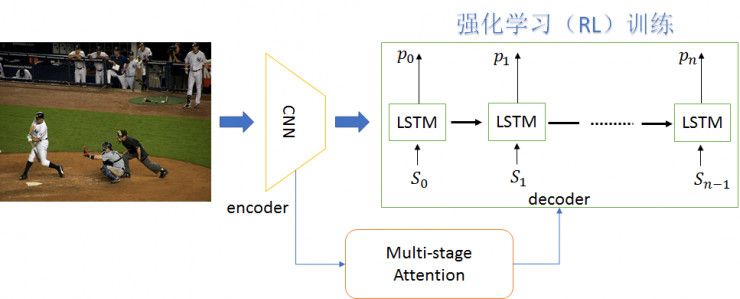
\includegraphics[scale=0.5]{Imgs/mdl.jpg}
	\caption{طرح‌واره‌ای از بستر کاری رمزگذار-رمزگشا}
	\label{fig:mdl}
\end{figure}

همان‌طور که قبلا ذکر شد، در این مدل، رمزگذار با دریافت تصویر، یک بردار ویژگی از تصویر استخراج می‌نماید و آن را به رمزگشا منتقل می‌نماید. رمزگشا که یک شبکه عصبی بازگشتی است، وظیفه تولید جمله متناظر تصویر را بر عهده دارد. به طور کلی این شبکه، در هر مرحله، احتمال رخ‌داد کلمه بعدی با توجه به بردار ویژگی تصویر و کلمات تولید شده قبلی را تولید می‌نماید. رابطه \eqref{eq:obj}، ساده‌ترین ارائه ریاضیاتی از این مدل را بیان می‌نماید که در آن، $\Phi_{t+1}$ خروجی شبکه بازگشتی در مرحله $t+1$، $\Theta$ بردار خروجی شبکه عصبی کانولوشنی و $y_0$ تا $y_t$  به ترتیب، کلمات تولید شده توسط شبکه عصبی بازگشتی در مراحل $0$ تا $t$ را نمایش می‌دهند.
\begin{equation}
	\Phi_{t+1} = p(y_{t+1} | y_0, y_1, \cdots, y_t, \Theta)
	\label{eq:obj}
\end{equation}

همان‌طور که مطابق با رابطه \eqref{eq:obj} مشخص است، خروجی شبکه، یک بردار به طول تعداد کلمات موجود در دیکشنری است که در هر مولفه آن، احتمال رخ‌داد کلمه متناظر در دیکشنری وجود دارد. کلمه خروجی در مرحله $t+1$ به شکل تصادفی و با توجه به این توزیع احتمال، از بین کلمات موجود در دیکشنری انتخاب می‌شود.
\\
فرایند آموزش این شبکه، به دلیل تنک بودن مقادیر خروجی مورد انتظارِِِ، تعداد پارامترهای زیاد و عدم استفاده از معنای لغات، فرایند سختی است. در این پژوهش ما از جاسازی کلمات\enfootnote{Word Embedding} استفاده کرده و مدل شبکه را از پیش‌بینی احتمال وقوع کلمات به انتخاب کلمه با معنای مورد انتظار تغییر دادیم. این کار باعث کاهش تعداد پارامترهای قابل آموزش شبکه، حذف برچسب‌های تنک و همین‌طور استفاده از معنای لغات و کلمات هم‌معنی در شرح تولیدی می‌شود. لازم به ذکر است، استفاده از جاسازی کلمات به جای پیش‌بینی احتمال رخ‌داد آن‌ها، نتایج بهتری را از خود نشان داده است.

\section{خلاصه فصول بعدی}
در این فصل سعی بر ارائه مقدمات اولیه پژوهش، بیان موضوع مساله، تاکید بر ضرورت حل مساله و بیان مختصری از سیر پژوهش‌های انجام شده در این حوزه داشتیم. در فصل‌ دوم از این گزارش، پژوهش‌های پیشین انجام شده در حوزه تولید شرح متناظر تصاویر را به طور مفصل مورد بررسی قرار می‌دهیم. در این فصل، علاوه بر ذکر مواردی از روش‌های قدیمی، بر روی بررسی پژوهش‌های انجام شده بعد از سال 2014 تمرکز بیشتری نموده و به دلیل ارتباط با ساختار استفاده شده در این پژوهش، ایده‌های مختلف ارائه شده در این سال‌ها را با جزئیات بیشتری بررسی می‌نماییم.
\\
در فصل‌ سوم، ایده اصلی پژوهش، ساختار و معماری شبکه‌های مورد استفاده و نحوه آموزش شبکه را مورد بررسی قرار خواهیم‌داد. فرایند آزمون و ارزیابی ساختار پیشنهادی را در فصل چهارم به طور کامل بررسی کرده و ضمن توضیح معیارهای ارزیابی مورد استفاده، نتایج عمل‌کرد روش پیشنهادی را با روش‌های دیگر ارائه شده، بیان می‌نماییم. لازم به ذکر است، بخش‌های اصلی کد پروژه، در پیوست اول آورده شده است.